\documentclass{article}

\usepackage{fancyhdr}
\usepackage{extramarks}
\usepackage{amsmath}
\usepackage{amsthm}
\usepackage{amsfonts}
\usepackage{tikz}
\usepackage[plain]{algorithm}
\usepackage{algpseudocode}
\usepackage[ngerman]{babel}

\usepackage[utf8]{inputenc}
\usepackage{amsmath}
\usepackage{amsthm}
\usepackage{amsfonts}
\usepackage{amssymb}
\usepackage{graphicx}


\usetikzlibrary{automata,positioning}

%
% Basic Document Settings
%

\topmargin=-0.45in
\evensidemargin=0in
\oddsidemargin=0in
\textwidth=6.5in
\textheight=9.0in
\headsep=0.25in

\linespread{1.1}

\pagestyle{fancy}
\lhead{\hmwkAuthorName}
\chead{\hmwkClass\ \hmwkClassInstructor\ \hmwkClassTime \hmwkTitle}
\rhead{\firstxmark}
\lfoot{\lastxmark}
\cfoot{\thepage}

\renewcommand\headrulewidth{0.4pt}
\renewcommand\footrulewidth{0.4pt}

\setlength\parindent{0pt}

%
% Create Problem Sections
%

\newcommand{\enterProblemHeader}[1]{
    \nobreak\extramarks{}{Aufgabenblatt \arabic{#1} continued on next page\ldots}\nobreak{}
    \nobreak\extramarks{Aufgabenblatt \arabic{#1} (continued)}{Aufgabenblatt \arabic{#1} continued on next page\ldots}\nobreak{}
}

\newcommand{\exitProblemHeader}[1]{
    \nobreak\extramarks{Aufgabenblatt \arabic{#1} (continued)}{Aufgabenblatt \arabic{#1} continued on next page\ldots}\nobreak{}
    \stepcounter{#1}
    \nobreak\extramarks{Aufgabenblatt \arabic{#1}}{}\nobreak{}
}

\setcounter{secnumdepth}{0}
\newcounter{partCounter}
\newcounter{homeworkProblemCounter}
\setcounter{homeworkProblemCounter}{1}
\nobreak\extramarks{Aufgabenblatt \arabic{homeworkProblemCounter}}{}\nobreak{}

%
% Homework Problem Environment
%
% This environment takes an optional argument. When given, it will adjust the
% problem counter. This is useful for when the problems given for your
% assignment aren't sequential. See the last 3 problems of this template for an
% example.
%
\newenvironment{homeworkProblem}[1][-1]{
    \ifnum#1>0
        \setcounter{homeworkProblemCounter}{#1}
    \fi
    \section{Aufgabenblatt \arabic{homeworkProblemCounter}}
    \setcounter{partCounter}{1}
    \enterProblemHeader{homeworkProblemCounter}
}{
    \exitProblemHeader{homeworkProblemCounter}
}

%
% Homework Details
%   - Title
%   - Due date
%   - Class
%   - Section/Time
%   - Instructor
%   - Author
%
%\newcommand{\hmwkTitle}{Aufgabe\ \#1}
\newcommand{\hmwkTitle}{Theoretische Informatik 1}
\newcommand{\hmwkDueDate}{}
\newcommand{\hmwkClass}{}
\newcommand{\hmwkClassTime}{}
\newcommand{\hmwkClassInstructor}{}
\newcommand{\hmwkAuthorName}{Dragan Runjaic , \\
				    Haris Ziko , \\
				    Peter Lorenz } 

%
% Title Page
%

\title{
    \vspace{2in}
    \textmd{\textbf{\hmwkClass:\ \hmwkTitle}}\\
    \normalsize\vspace{0.1in}\small{Due\ on\ \hmwkDueDate\ at 3:10pm}\\
    \vspace{0.1in}\large{\textit{\hmwkClassInstructor\ \hmwkClassTime}}
    \vspace{3in}
}

\author{\textbf{\hmwkAuthorName}}
\date{}

\renewcommand{\part}[1]{\textbf{\large Part \Alph{partCounter}}\stepcounter{partCounter}\\}

%
% Various Helper Commands
%

% Useful for algorithms
\newcommand{\alg}[1]{\textsc{\bfseries \footnotesize #1}}

% For derivatives
\newcommand{\deriv}[1]{\frac{\mathrm{d}}{\mathrm{d}x} (#1)}

% For partial derivatives
\newcommand{\pderiv}[2]{\frac{\partial}{\partial #1} (#2)}

% Integral dx
\newcommand{\dx}{\mathrm{d}x}

% Alias for the Solution section header
\newcommand{\solution}{\textbf{\large Solution}}

% Probability commands: Expectation, Variance, Covariance, Bias
\newcommand{\E}{\mathrm{E}}
\newcommand{\Var}{\mathrm{Var}}
\newcommand{\Cov}{\mathrm{Cov}}
\newcommand{\Bias}{\mathrm{Bias}}






\begin{document}
%\maketitle
%\pagebreak
 
 \newcommand{\TM}{\xrightarrow[\tau]{1}}
 \newcommand{\TMM}{\xrightarrow[\tau]{*}}
 
.  \newline
\begin{homeworkProblem}
  \subsection{1. Entwerfen Sie eine deterministische 1-Band Turingmaschine die COUNT entscheidet.}

    \begin{figure}[htbp]
      \centering
      \fbox
      {
	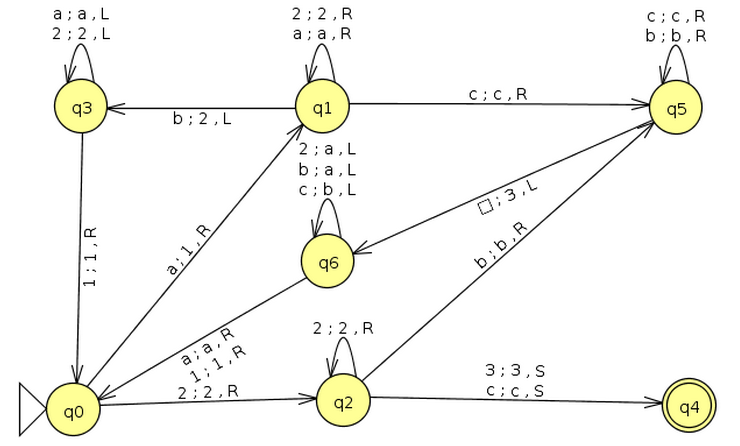
\includegraphics[width=0.7\textwidth]{Abbildung_1.png}
      }
      \caption{Turingmaschine}
      \label{Labelname}
    \end{figure}
  
    Unser Programm arbeitet in zwei Teilen. Die Zustände $q_0$, $q_1$ und $q_3$ stellen fest ob sich im ersten gleich viele a-Symbole,
    wie b-Symbole befinden. Der zweite Teil der Turingmaschine, also die Zustände $q_0$, $q_2$, $q_5$ und $q_6$, führen den Vergleich
    der Anzahl von b- mit c-Symbolen auf einen Vergleich von a- mit b-Symbolen zurück und führt somit, das Problem auf den ersten Teil
    unserer Turingmaschine zurück.\\
      
    % Zu Beginn sind wir im Zustand $q0$. Auf dem Band muss ein $‘a’$ stehen, was zu dem 
    % Eingabealphabet  gehört. Die DTM kontrolliert zu erst, ob die Zeichenfolge a und b die gleich oft vorkommen. $‘c’$  wird vorerst ignoriert. 
    % Das erste $‘a’$ wird überschrieben mit einem  $‘1‘$, somit hat man es markiert und hat sich gemerkt, dass sie schon mal da war. Nun wird das nächste $‘b’$ 
    % gesucht und mit einer  $‘2‘$ überschrieben. Wenn gleich viele $‘a’$ wie $‘b’$s vorkommen, dann terminiert die DTM vorzeitig. 
    % Falls das nicht eintrifft, dann werden die jetzigen  $‘2‘$er und $‘b’$s ersetzt mit $‘a’$ und die $‘c’$ mit $‘b’$. Nach dem letzten $c$ wird eine $3$ angehängt, 
    % damit man das Ende des Bandes markiert. \\
    % Die DTM arbeitet wieder gleich weiter, wie oben im ersten Absatz beschrieben, da die $‘a’$ und $‘b’$ als richtige Symbole gegeben sind. Wenn gleich viele $‘b’$
    % wie $‘c’$ vorhanden sind, dann terminiert und entscheidet COUNT. \\

  
  
  \subsection{2. Beweisen Sie formal, dass diese Maschine korrekt funktioniert, d.h. dass sie genau dann den Endzustand erreicht, wenn die Eingabe aus $COUNT$ ist.} 
    
    Unser Alphabet beinhaltet $ \Sigma = \{a,b,c,1,2,3\} $. Wir definieren außerdem für $ m\in\mathbb{N} $.
    \begin{center}
      $ \alpha_m = \underbrace{aa\dots a}_{m},
      \beta_m = \underbrace{bb\dots b}_{m}, 
      \gamma_m = \underbrace{cc\dots c}_{m}, 
      \sigma_m = \underbrace{11\dots 1}_{m}, 
      \rho_m = \underbrace{22\dots 2}_{m} $ 
    \end{center}
    
    Wir betrachten ein zu überprüfendes Wort $w = \alpha_i\beta_j\gamma_k$ wobei $i, j, k > 0$. \\
    
    \underline{Erster Teil(Vergleichen)} 
    \begin{figure}[htbp]
      \centering
      \fbox
      {
	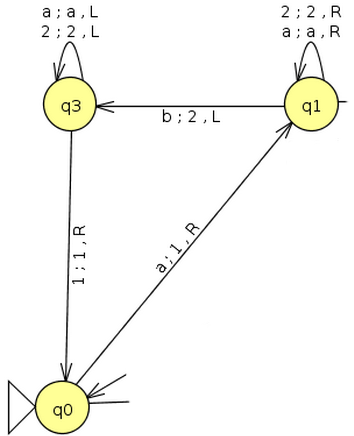
\includegraphics[width=0.2\textwidth]{Abbildung_2.png}
      }
      \caption{Vergleichen}
      \label{Labelname}
    \end{figure}
    
    Wie oben bereits beschrieben vergleicht der erste Teil nur die a-Symbole mit den b-Symbolen, daher betrachten
    wir nur den ersten Teil des Wortes ohne die c-Symbole.
    
    $$w = \{\alpha_i\beta_j\}$$
      
      
    \begin{enumerate}
      \item Fall: \textbf{i=j} \quad Beispiel: ab  % https://www.sharelatex.com/learn/Spacing_in_math_mode
      \begin{itemize}
	\item \textbf{Basis:} $ q_0 ab \TM  1 q_1 b \TM  q_3 2 \rightarrow q_0 12 $ 
	\item \textbf{Vorraussetzung:} $ q_0 \alpha_{i} \beta_{j} \xrightarrow{*} q_0 \sigma_{i} \rho_{j} $ 
	\item \textbf{Schritt:} ($ i \rightarrow i + 1 $) \\
	$ q_0 \alpha_{i+1} \beta_{j+1} \equiv q_0 \alpha{i} \beta_j b \TMM q_1 \sigma_i a \rho_j b $
	$ \TM q_3 \sigma_i 1 \rho_j b \TM q_0 \sigma_{i+1} \rho_{j+1} $ 
      \end{itemize}
    
      \item Fall:  \textbf{i\textgreater j} für j \textgreater 0  und i = j + 1 ... n. Beispiel: $ aaaab \rightarrow 11aa2 $
      \begin{itemize}
	\item \textbf{Basis:} $q_0 aab \TM 1 q_1 ab \TMM 1 a q_3 2 \TM q_0 1a2 \TM 11 q_1 2 (\TMM 112 q_5) $
	\item \textbf{Vorraussetzung:} $ q_0 \alpha_i \beta_j \TMM \sigma_{j+1} \alpha_{i-j-1} q_1 \rho_j $
	\item \textbf{Schritt:} $ q_0 \alpha_{i+1} \beta_j \equiv q_0\alpha_i a \beta_j \TMM \sigma_{j+1} \alpha_{i-j-1} 
	a q_1 \rho_j \equiv \sigma_{j+1}\alpha_{i-j} q_1 \rho_j  \rightarrow (\sigma_{j+1}\alpha_{i-j}\rho_j q_5)  $
      \end{itemize}	
      
      \item Fall:  \textbf{i\textless j} Schneide ab, sodass i=j. Beispiel: $ abbb \rightarrow 12bb $ \\
	Betrachte Teilwert mit $w = \alpha_i \beta_i \longrightarrow Fall 1$

    \end{enumerate}
    
    Wir sehen also, dass man Im Fall 1 über den Zustand $q_2$ (Die c-Symbole werden hier nur überspult)
    in den Endzustand kommt. Im Fall 2 landen wir über Zustand $q_2$ (Ein b-Symbol, dass ja vorhanden sein muss,
    da im Fall 2 $j>i$ war, wird überspult) in $q_5$.
    Im Fall 3 landen wir direkt im Zustand $q_5$ und somit im zweiten Teil unserer
    DTM (siehe unten). \\

    \underline{Zweiter Teil(Überschreiben)} 
    \begin{figure}[htbp]
      \centering
      \fbox
      {
	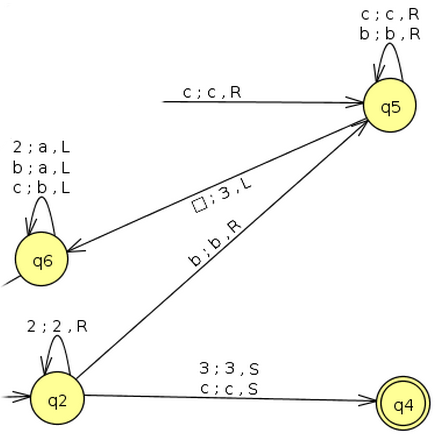
\includegraphics[width=0.2\textwidth]{Abbildung_3.png}
      }
      \caption{Überschreiben}
      \label{Labelname}
    \end{figure}
    Hier wird in $q_5$ bis ans rechte Bandende gespult und anschließend zur Wiedererkennung ein 3-Symbol
    ans rechte Bandende gesetzt. Der nachfolgende $q_6$ Zustand überschreibt alle c-Symbole mit b-Symbolen
    und alle 2/b-Symbole mit a-Symbolen während er wieder nach links Spult bis er ein 1 oder a-Symbol findet
    und im Zustand $q_0$ landet. Hier wird wieder der erste Teil(Vergleichen) aufgerufen.
    
    Falls im zweiten durchlauf von (Vergleichen) keine Übereinstimmung gefunden wird, so entscheidet
    das Programm ein Wort nicht und bleibt im Zustand $q_5$ stecken. \\
    

  \subsection{3. Laufzeitanalyse der TM und z.z. $COUNT \in P$ } 
    
    \underline{Analyse des ersten Teils (Vergleich von a- und b-Symbolen):} 
    
    Die DTM überschreibt a-Symbole mit 1-Symbolen und der Lesekopf bewegt sich dann zum ersten b-Symbol, welches er mit dem 2-Symbol ersetzt
    und anschließend wandert er zurück zum nächsten a-Symbol. Diesen Prozess wiederholt die DTM so lange, bis alle a- und b-Symbole mit den
    entsprechenden 1- bzw 2-Symbolen ersetzt wurden. Falls es gleich viele sind geht die DTM in den Endzustand über, ansonsten in den zweiten
    Teil unserer DTM ( siehe unten ).
    
    Den Abstand,den der Lesekopf zurücklegt, jedes Mal wenn er von a nach b bzw von b nach a bewegt, ist klarerweise $\leq n$ und er legt diese
    Distanz maximal $n$ mal zurück. ( Im worst case, also wenn $i=j$, $i \leq n$ mal ) Daher ergibt sich für den ersten Teil eine Laufzeit von 
    
    $$T(n) = \mathcal{O}(n)*\mathcal{O}(n) = \mathcal{O}(n^2)$$ \\
    
    \underline{Analyse des zweiten Teils (Zurückführung des c-,b-Problems auf den ersten Teil)}
    
    Dieser Teil der DTM wird nur dann aufgerufen, falls der erste Teil nicht entschieden worden ist ( und somit $i \neq j$ ). Nun gilt zu überprüfen,
    ob die Anzahl der b-Symbolen gleich der Anzahl der c-Symbolen ist ( daher ob $j = k$ ). Die DTM beginnt vom rechten Bandende zu arbeiten und
    und ersetzt der Reihe nach alle c-Symbole mit b-Symbolen und alle 2-Symbole/b-Symbole (die ja vorher b-Symbole waren) mit a-Symbolen, bis 
    der Lesekopf ein 1-Symbol erreicht. Dieser Prozess findet nur einmal statt, denn nun befindet sich die DTM wieder im ersten Teil. Die Laufzeit
    für den zweiten Teil ergibt sich also nur durch das einmalige Zurücklegen der Distanz vom rechten Bandende bis zum ersten 1-Symbol. Daher:
    
    $$T(n) = \mathcal{O}(n)$$ \\
    
    Als \textbf{resultierende Laufzeit} für die gesamte DTM ergibt sich damit:
    
    $$T(n) = \mathcal{O}(n^2) + \mathcal{O}(n) = \mathcal{O}(n^2)$$
    
    \vfill
    \begin{verbatim}
      Literatur: 
      http://www.igi.tugraz.at/lehre/TI1/SS15/ue/TI1-UE-03-handout.pdf
    \end{verbatim}
    
\end{homeworkProblem}

\pagebreak

\begin{homeworkProblem}
    \subsection{1. Beweisen, Sie dass ein perfektes Matching in diesem Graphen mit $|A| = |B| = k$ genau dan existiert, wenn $max_{f} F(f) = k$.}
    
    
Der Beweis gliedert sich in zwei Teile. \\

\underline{Zunächst beweisen wir, dass aus $\max_f F(f) = k$ folgt, dass es ein perfektes Matching gibt:}\\


Wir nehmen also zunächst an $\max_f F(f) = k$, daher also in unserem bipartiten Graphen existiert ein Fluss $f^*$, der genau den Flusswert $k$ besitzt. Da $|A| = |B| = k$ gilt, folgt

\begin{equation}
F(f^*) = \sum_{i=1}^k f^*((q,a_i)) = \sum_{i=1}^k f((b_i,s)) = k, \quad a_i \in A, b_i \in B
\label{bsp2:1}
\end{equation}

wobei $q$ und $s$ die in der Angabe definierte Quelle und Senke ist. Betrachten wir nun die Kapazitäten der Kanten $0 \leq f((i,j)) \leq 1, \forall (i,j) \in E$ (und für alle Flüsse $f$) so sehen wir, dass

\begin{equation}
f((q,a_i)) = f((b_i,s)) = 1 \quad \forall i=1,\dots,k
\end{equation}

gelten muss, da in (\ref{bsp2:1}) die Summe $k$ Summanden hat, die zwischen Null und Eins liegen und somit nur den Wert $k$ annehmen kann falls alle Summanden den Wert Eins annehmen. \\

Angenommen es existiert nun kein perfektes Matching (Daher $2|M| < |V|$) in unserem Graphen $G=(V,E)$. Da es sich um einen bipartiten Graphen handelt existiert innerhalb von $B$($A$) keine Kante, die Knoten von $B$($A$) mit sich selbst verbindet. Damit nun kein perfektes Matching existieren kann, unterscheiden wir zwei Fälle:

\begin{enumerate}
\item Es gibt mindestens einen Knoten $w \in B(A)$, der mit keiner Kante aus $A$($B$) verbunden ist. Dies führt aber sofort zu einem Widerspruch zur Flusserhaltungsbedingung ,denn

\begin{equation}
0 = \sum_{p \in Parent(w)} f((p,w)) = \sum_{c \in Child(w)} f((w,c)) = f((w,s)) = 1
\end{equation}

\item O.B.d.A betrachten wir $B$. Alle Knoten aus $B$ sind mit einer Kante aus $A$ verbunden und es gibt mindestens einen Knoten $w \in B$, der nicht gematcht wird. Dies bedeutet aber, dass er mit einem Knoten $v \in A$ verbunden sein muss der gemacht wird, denn ansonsten könnte man diese Kante zum Matching hinzufügen und somit erweitern (Führt man dies iterativ weiter so bekommt man ein perfektes Matching). Da der Knoten $v$ im Matching ist, muss er mit einem anderen Knoten $w' \in B, w \neq w'$ verbunden sein. Diese drei Knoten $w,v,w'$ können aber nicht die Flusserhaltungsbedingung aufrecht erhalten, denn aus $w$ und $w'$ fließen jeweils 1 ab aber in $v$ können nicht 2 einfließen. Damit muss es also noch einen weitere Kante geben die mit Pfad $(w,v,w')$ verbunden ist. Falls diese Kante aus vorherigen Überlegungen nicht in $w$ führen und auch nicht aus $v$ hinausführen, denn sonst müsste in den Knoten $v$ 3 Einheiten einfließen. Also muss eine Kante $(v',w'), v'\in A$ in $w'$ führen und diese kann keine Matchingkante sein, da $(v,w')$ eine Matchingkante ist. Nun haben wir einen Pfad $(w,v,w',v')$, wobei $(w,v)$ und $(w',v')$ keine Matchingkanten sind aber $(v,w')$ eine Matchingkante ist. Tauschen wir die Rollen der Kanten so erhalten wir ein Matching mit einer neuen Matchingkante. Setzten wir hier iterativ fort ist dies ein Widerspruch zu $2|M| < |V|$.
\end{enumerate} 

Zusammengefasst, war also die Annahme es existiere kein perfektes Matching falsch und es muss daher eines existieren. \\

\underline{Nun beweisen wir, wenn ein perfektes Matching existiert, so gilt $\max_f F(f) = k$:}\\

Wir nehmen an, es existiert ein perfektes Matching $M^*$ und konstruieren einen Fluss $f^*$ der den Wert $F(f^*) = k$ besitzen wird. Dazu setzten wir

\begin{equation}
f^*((a,b)) = \left\{\begin{array}{cl} 
1, & \mbox{falls }(a,b) \in M^*\\ 
0, & \mbox{sonst} \end{array}\right. 
\quad \forall a\in A,b \in B.
\end{equation}

Dies bedeutet zwischen einem Knoten $a\in A$ und einem Knoten $b \in B$ existiert genau eine Kante, nämlich die Matchingkante, die genau eine Flusseinheit transportiert. Setzten wir nun $f^*((q,a)) = 1, \forall a \in A$ und $f^*((b,s)) = 1, \forall b \in B$, so
gilt offensichtlich 

\begin{equation}
\sum_{p \in Parent(v)} f^*((p,v)) = \sum_{c \in Child(v)} f^*((v,c)) = 1.
\end{equation}

Dies bedeutet wir haben einen zulässigen Fluss konstruiert, der den Wert

\begin{equation}
F(f^*) = \sum_{i=1}^k f^*((q,a)) = \sum_{i=1}^k 1 = k.
\end{equation}

Somit muss also $\max_f F(f) \geq k$ gelten. Da allerdings $0 \leq f((i,j)) \leq 1, \forall (i,j) \in E$ gilt, muss $\max_f F(f) \leq k$ sein, da maximal $k$ Kanten in $s$ münden bzw aus $q$ ausgehen. Daraus folgt
\begin{equation}
\max_f F(f) = k
\end{equation} 
    
    \subsection{2. Beweisen, Sie dass jeder (endliche) DAG zumindest eine Quelle und eine Senke hat.}
    
Nehmen wir zunächst an, es existiere ein DAG $G=(V,E)$, der keine Quelle und Senke besitzt. Dies bedeutet er muss in jedem Knoten $v\in V$ mindestens eine eingehende und eine ausgehende Kante besitzen, denn sonst wäre er eine Quelle bzw. Senke. Dies bedeutet aber das eine Folge von Knoten $v_1, \dots, v_k \in V$ existieren muss, sodass es von $v$ einen Weg zu sich selbst, also $v$ geben muss, da ansonsten ja eine Quelle existieren müsste die einen Weg zu $v$ besitzt. Dieser Weg $(v,v_,\dots,v_k,v)$ ist aber per Definition ein Kreis und somit ein Widerspruch zur Azyklizität von unserem Graphen. Somit war unsere Annahme falsch und es muss mindestens eine Quelle und eine Senke existieren.
    
    
\end{homeworkProblem}

    
    
\pagebreak

\begin{homeworkProblem}
   
    \subsection{1. Zu Zeigen: Jede DTM kann mit polynomiellem Zeitaufwand auf einem determnistischen Warteschlangen-Automat simuliert werden, und umgekehrt.}

    % todo
    Damit man eine DTM auf eine oder mehrere DWA's zu simulieren, sind die Bewegungsmöglichkeiten 
    der beiden zu beachten:
    \begin{itemize}
     \item \textbf{DTM:} liest ein Symbol und kann sich der Lesekopf nach link oder rechts bewegen, dann ein 
      Symbol schreiben und den Zustand wechseln.
     \item \textbf{DWA:} Pop, Push und Zustandsänderung.
    \end{itemize}
    
    \underline{Um die Äquivalenz zwischen dem DWA und DTM zu zeigen, müssen wir 2 Fälle behandeln:}
    \begin{enumerate}
     \item \textbf{DWA auf DTM:} 
     
      DWA und DTM haben die selbe Eingabe. Das erste Symbol dient zur Erkennung,
      wo die Angabe anfängt. Wir wollen nun die Eingabe zyklich verschieben. \\
      DWA: Wenn man bei der DWA ein Symbol popped und das gleiche Symbol wiederum pushed, solange bis
      das erste Symbol erreicht wird und wieder die die selbe Eingabe im DWA steht. 
      $$ T(n) = \mathcal{O}(1) + \mathcal{O}(1) = \mathcal{O}(1) $$
      
      DTM: Der Lesekopf bewegt sich vom ersten Symbol bis zum ersten Blanksymbol, damit das letzte 
      Symbol erkannt wird, geht er wieder einen Schritt nach links. Das an dieser Stelle stehende Symbol
      wird gelesen und mit einem Blanksymbol überschrieben. Der Lesekopf wandert wiederum ganz nach rechts
      bis zum ersten Blanksymbol, wo das gelesene Symbol platziert wird. Nun bewegt sich der Kopf nach rechts und
      holt sich das nächste Symbol, solange bis das erste Symbol gelesen wird. 
      $$ T(n) = \mathcal{O}(n) + \mathcal{O}(n) = \mathcal{O}(n) $$
      
     \item \textbf{DTM auf DWA:}
     
     DTM: Es gibt um die Verschiebung(Lesen|R|Schreiben) des Lesekopfes der DTM, die dann auf der DWA gezeigt soll werden.
     $$ T(n) = \mathcal{O}(1) $$
     
     DWA: Um diese Verschiebung auf einem DWA zu zeigen, werden zwei weitere Symbole eingeführt. Das eine repräsentiert
     die Schreib/Lese Kopf und das andere steht ganz am Ende des DWA`s, was das Ende repräsentiert. 
     Die ersten zwei Symbole werden popped und das zweitere anschließend gepushed und danach das erste Symbol.
     Danach kommen alle anderen Symbole und der Reihe nach popped und pushed.
     $$ T(n) = \mathcal{O}(1) + \mathcal{O}(n) = \mathcal{O}(n) $$
     
    \end{enumerate}

    \newpage
    
    \subsection{2. Zu Zeigen: Ein deterministischer 2-KA ist mächtiger als ein deterministischer 1-KA.}
    
    % todo
    Um zu zeigen, dass der 2-KA mächtiger ist als der 1-KA, muss eine Sprache existieren, die am 1-KA nicht entscheidet. 
    Wir stellen hier zwei den 1-KA udn 2-KA gegenüber: \\
    
    Der 1-KA Automat kann nicht entscheiden, ob ein Palindrom (Chomsky Hierarchie: Typ 2) gültig ist:  
    
    \begin{figure}[htbp]
      \centering
      \fbox
      {
	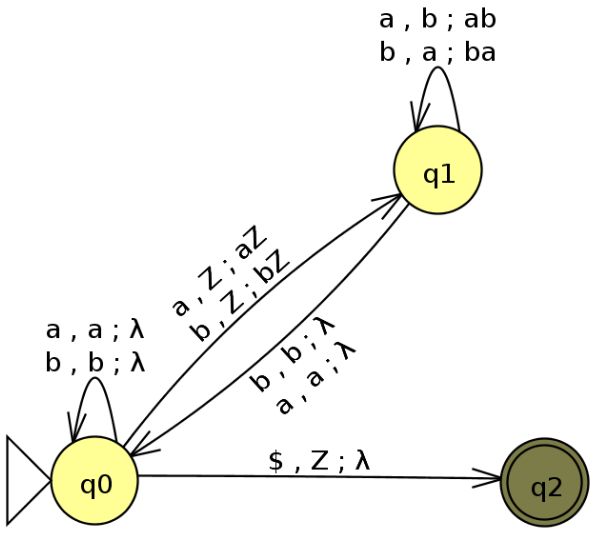
\includegraphics[width=0.4\textwidth]{Abbildung_4.png}
      }
      \caption{1-KA}
      \label{Labelname}
    \end{figure}
 
    $\Sigma = { a, b, Z, \$, \lambda }$, wobei das \$-Symbol zur Markerierung vom Ende der Eingabe dient und 
    das Z-Symbol das Ende im Stack markiert.
    Vom Zustand $q_0$ auf $q_1$ wird geprüft, ob die Eingabe aus Teilpalindromen enthält. Teilpalindrome sind Symbole aus
    der Kombination von $ab$ und $ba$, die zwischen Stack und Eingabe verglichen werden. 
    Das Problem des 1-KA ist, dass nicht die gesamte Eingabe betrachtet wird sondern die 
    eben zuvor erwähnten Kombinationen. Folglich können mehrere Palindrome zusammen in die Eingabe sein, was dann der 
    1-KA entscheidet, obwohl er nicht sollte. 
    
    \pagebreak
    \begin{figure}[htbp]
      \centering
      \fbox
      {
	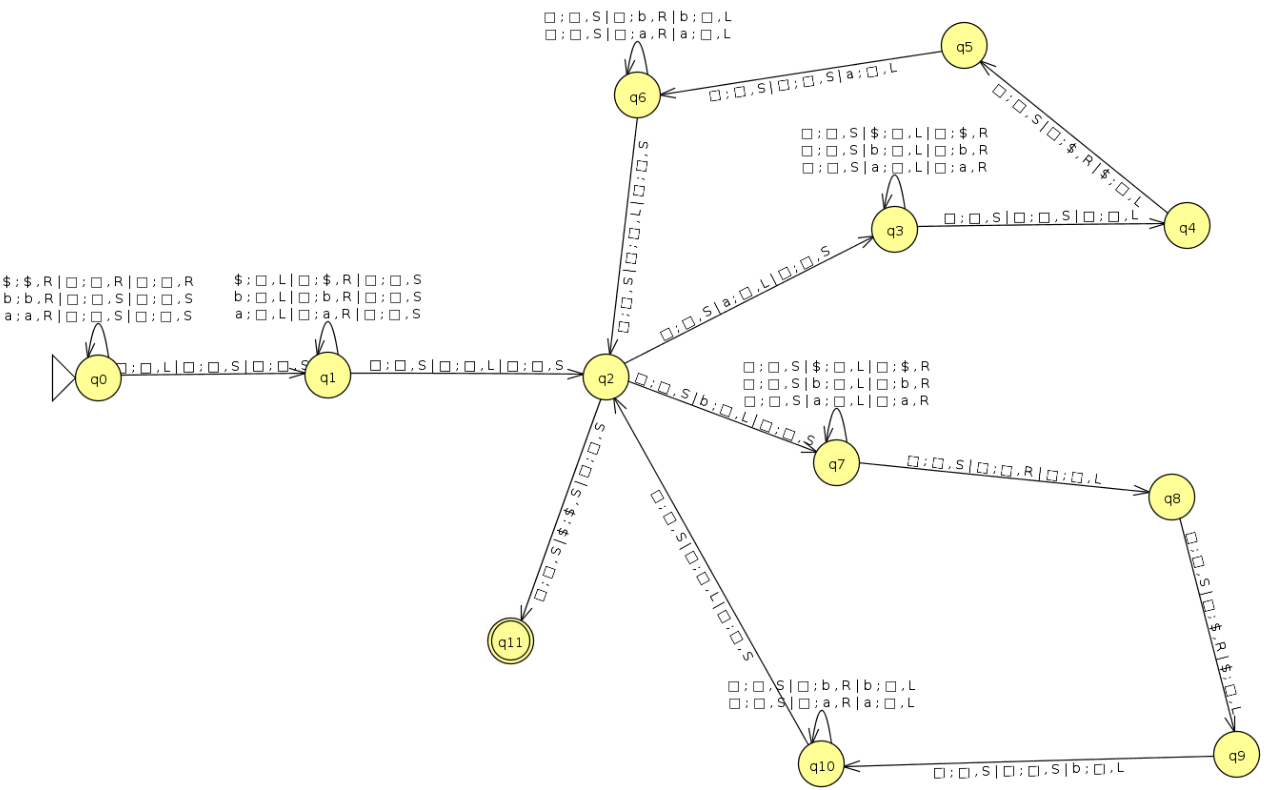
\includegraphics[width=0.9\textwidth]{Abbildung_5.png}
      }
      \caption{Simulation von 2-KA auf eine 3-DTM}
      \label{Labelname}
    \end{figure}
    
    In Abbidlung 5 wird einen 2-KA auf eine 3-DTM simuliert (da es in JFLAP für 2-KA nicht realisierbar ist). 
    Auf dem ersten Band findet man die Eingabe, und die zwei weiteren Bänder dienen als Stacks. 
    Es wird vom ersten Band alle Symbole auf das zweite Band geschrieben. Die Abbildung 5 hat grundsätzlich
    zwei Schleifen, die eine arbeitet die a-Symbole und die andere die b-Symbole ab.
    Vom ersten Stack wird das erste Symbol gelesen und gelöscht, jedoch wird das Symbol anhand eines Zustandes 
    gemerkt. \\
    Die restlichen Symbole werden auf Band 2 geschrieben und nun nach dem \$-Symbol, was das Ende(Band 1) bzw. Anfang
    (Band 2) zeigt, muss wieder das gleiche Symbol (letzte) folgen, welches vorhin gelöscht wurde. 
    Nun beginnt das ganze wieder von vorne so lange bis alle Symbole abgearbeitet wurden. \\
    
    
    Der 2-KA betrachtet somit die gesamte Eingabe und kann entscheiden, ob die Eingabe ein Palindrom ist.
    Als Resulat kann der 2-KA in der Chomsky Hierarchie die Sprachen vom Typ 2 lösen und ist daher 
    mächtiger als ein 1-KA. 
    
    
    
    
    
    
    
    \vfill
    \begin{verbatim}
    Literatur:
      http://en.wikipedia.org/wiki/Queue_automaton 
      http://www.igi.tugraz.at/lehre/TI1/SS15/vo/TI1-VO-02-handout.pdf
    \end{verbatim}
  
    
\end{homeworkProblem}


\end{document}